
\documentclass[12pt, a4paper]{article}

%-----------USEPACKAGE----------------------------
\usepackage{bm} % Tucne pismo
\usepackage[czech]{babel} % Cestina
\usepackage[T1]{fontenc}
\usepackage[utf8x]{inputenc}
\usepackage[unicode]{hyperref} % Odkazy v pdf, www a na e-mail
\usepackage{graphicx} % Obrazky
\usepackage{epstopdf} % Obrazky
\linespread{1.10} % Radkovani 1.3 odpovida radkovani 2
\usepackage{lmodern} % Daji se pouzit \HUGE atd.
\usepackage{amsmath}
\usepackage{algorithm}
\usepackage[noend]{algpseudocode} % Vkladani pseudo kodu
\usepackage{color}
\usepackage{listings}
\usepackage{setspace}

%-----------COLORS--------------------------------
\definecolor{Code}{rgb}{0,0,0}
\definecolor{Decorators}{rgb}{0.5,0.5,0.5}
\definecolor{Numbers}{rgb}{0.5,0,0}
\definecolor{MatchingBrackets}{rgb}{0.25,0.5,0.5}
\definecolor{Keywords}{rgb}{0,0,1}
\definecolor{self}{rgb}{0,0,0}
\definecolor{Strings}{rgb}{0,0.63,0}
\definecolor{Comments}{rgb}{0,0.63,1}
\definecolor{Backquotes}{rgb}{0,0,0}
\definecolor{Classname}{rgb}{0,0,0}
\definecolor{FunctionName}{rgb}{0,0,0}
\definecolor{Operators}{rgb}{0,0,0}
\definecolor{Background}{rgb}{1, 1, 1}

%-----------LISTINGS-SETTINGS----------------------
\lstset{
	numbers=left,
	numberstyle=\footnotesize,
	numbersep=0.5em,
	xleftmargin=1.5em,
	xrightmargin=0em,
	framextopmargin=0em,
	framexbottommargin=0em,
	showspaces=false,
	showtabs=false,
	showstringspaces=false,
	frame=lrtb,
	tabsize=4,
	% Basic
	basicstyle=\ttfamily\footnotesize\setstretch{1},
	backgroundcolor=\color{Background},
	language=Python,
	% Comments
	commentstyle=\color{Comments}\slshape,
	% Strings
	stringstyle=\color{Strings},
	morecomment=[s][\color{Strings}]{"""}{"""},
	morecomment=[s][\color{Strings}]{'''}{'''},
	% Keywords
morekeywords={import,from,class,def,for,while,if,is,in,elif,else,not,and,or,print,break,continue,return,True,False,None,access,as,del,except,exec,finally,global,import,lambda,pass,print,raise,try,assert},
	keywordstyle={\color{Keywords}\bfseries},
	% Additional keywords
	morekeywords={[2]@invariant},
	keywordstyle={[2]\color{Decorators}\slshape},
	emph={self},
	emphstyle={\color{self}\slshape},
	breaklines=true, % Zalamuje radky.
}






%------------------VARIABLES----------------------------
\newcommand{\cisloZadani}{Zadání semestrální práce - 3}









%------------------LAYOUT----------------------------
\usepackage[top = 2.5 cm, bottom = 2.5 cm, left = 2.5 cm, right = 2.5 cm]{geometry} % geometrie stranky
\usepackage{longtable}% Pro dlouhy obsah, da se zalomit \pagebrek
\usepackage{fancyhdr}
\pagestyle{fancy}% Deffaultni nastaveni hlavicky a paticky
\setlength{\headheight}{16 pt}% Zvetsi hlavicku, aby to nedelalo warningy
\fancyhf{}
\lhead{\href{http://www.kky.zcu.cz/cs/courses/mpv}{Metody Počítačového Vidění}}
\rhead{\cisloZadani}
\fancyfoot[R]{\thepage}
\fancyfoot[L]{Verze 1.0.0, poslední úpravy: \today}








%---------------BEGIN-DOCUMENT--------------------------
\begin{document}
 









 
%--------TITLE-PAGE--------------------------------------------
\begin{titlepage}
\begin{center}
	
\includegraphics[trim = 0.6cm 0.5cm 0.9cm 0.5cm, scale=1]{./FAV_logo_cz.pdf}
	\hspace*{\fill}
	
\includegraphics[trim = 3.5cm 1.5cm 2.6cm 2cm, scale=0.295]{./KKY_logo_cz.pdf}\\
	\vspace*{\fill}
	\textbf{\Huge{\href{http://www.kky.zcu.cz/cs/courses/mpv}{Metody Počítačového Vidění} \\ ~ \\ \cisloZadani}}\\
	\vspace*{\fill}
	\textbf{\large{\href{mailto:LBures@kky.zcu.cz}{Ing. Lukáš Bureš}}} \hfill \textbf{\large{Plzeň, \today}}
\end{center}
\end{titlepage}








%-------------------------------------------------------------
\section*{\cisloZadani}

\par{Cílem semestrální práce je \textbf{klasifikovat ručně psané číslovky} do odpovídající třídy. Je žádoucí vymyslet a vytvořit vhodný popis vstupních trénovacích obrázků, který bude využit jako příznakový vektor pro natrénování Support Vector Machines (SVM) klasifikátoru.}

\par{\textbf{Vstup:} Vektor obrázků o rozlišení $20 \times 20$ pixelů.}

\par{\textbf{Výstup:} Vektor s hodnotami tříd, do kterých byl vstupní obrázek klasifikován a dále OpenCV SVM objekt klasifikátoru.}

\par{\textbf{Ohodnocení:} Za bezchybně vypracovanou semestrální práci lze získat \textbf{až 25\%} z~celkového hodnocení ze semestru.}

\par{\textbf{Deadline:} Den před cvičením v 11. týdnu zimního semestru ve 23:59:59 hodin.}

\par{\textbf{Poznámka:} Není povoleno využít známé implementace volně dostupné na internetu. Práce bude po deadlinu kontrolována na \textbf{plagiátorství} a nevyhovující práce budou ohodnoceny \textbf{0\%}! Je očekávána vlastní implementace algoritmu.}

\section*{Informace a doporučení}
\begin{enumerate}
	\item Vstupní data jsou vidět na Obr. \ref{fig:Train}, kde jednotlivé číslice jsou tvořeny podobrázkem o velikosti $20 \times 20$ pixelů. Zařazení do třídy odpovídá číslovce, například pokud je na obrázku číslovka 2, tak bude patřit do třídy 2. Vstupní data tvoří $70\%$ celé množiny dat.
	\item Je možné využít například $20\%$ ze získaných dat jako \href{http://en.wikipedia.org/wiki/Cross-validation_(statistics)}{\textit{cross validation sadu}}. 
	\item Je doporučeno obrázky pomocí předzpracování vhodně normalizovat.
	\item Získejte vhodný popis obrázku jednotlivých číslovek (příznakový vektor).
	\item Natrénujte SVM klasifikátor z příznakových vektorů.
	\item Použijte implementaci SVM z OpenCV.
	\item \textbf{Upozornění:} SVM klasifikátor může být trénován pouze z dodaných dat!
\end{enumerate}

\pagebreak

\begin{figure}[ht!]
	\centering
	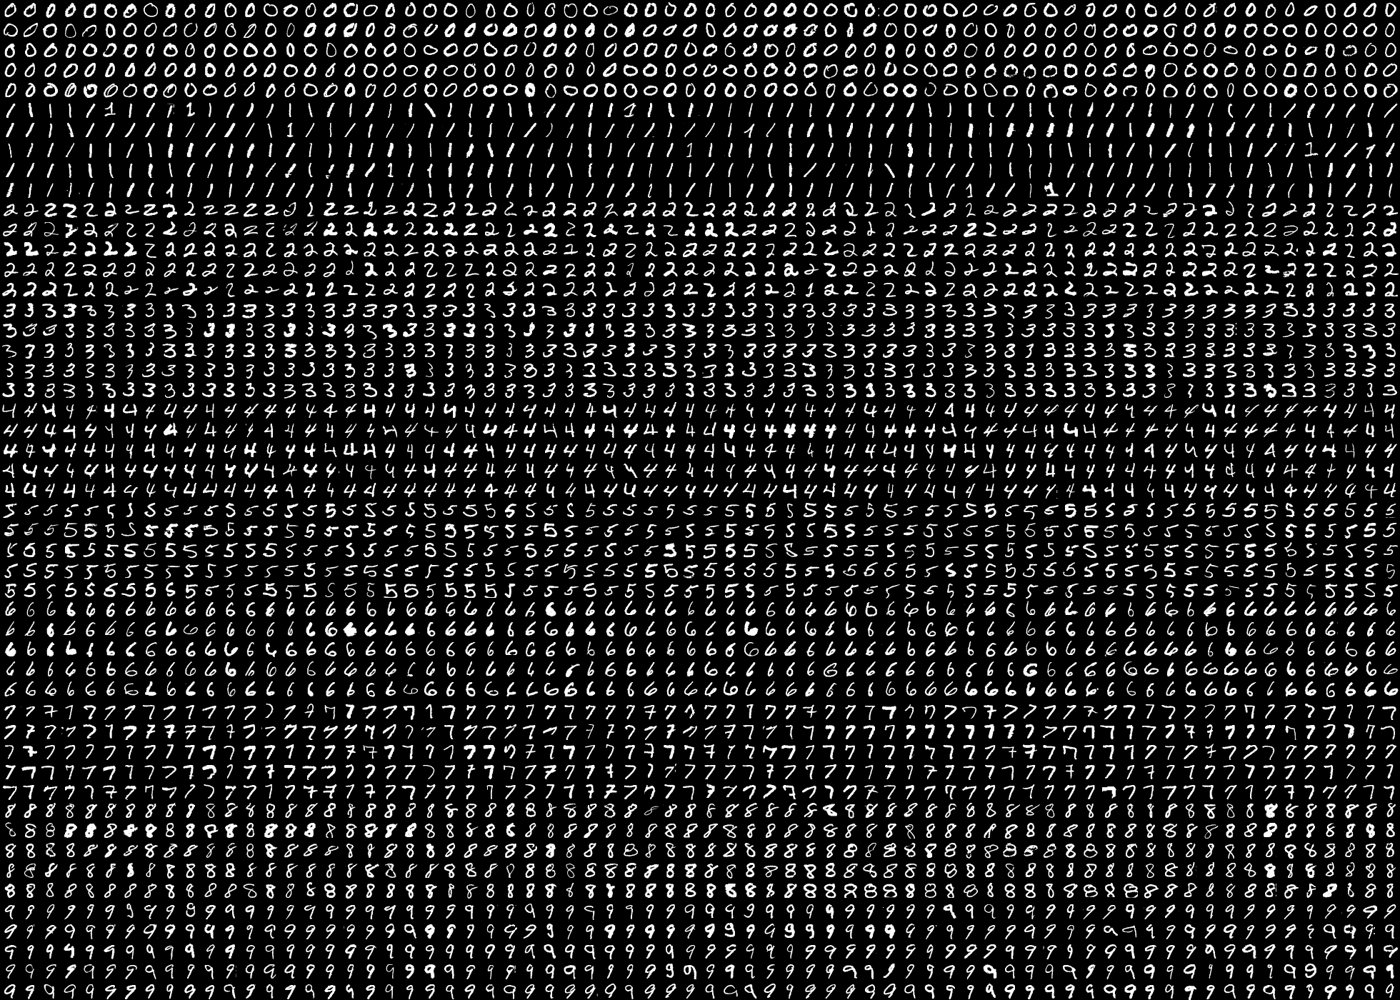
\includegraphics[width=\textwidth]{Train.png}
	\caption{Vstupní data ručně psaných čísel.}
	\label{fig:Train}
\end{figure}			


\section*{Doporučená literatura}
\begin{enumerate}
	\item Přednášky a učební materiály MPV.
	\item \href{http://docs.opencv.org/}{Dokumentace k OpenCV}
\end{enumerate}



\end{document}



















